\begin{comment}

In order to complete the work required to meet my aims, various pieces of software, tools and methods will be required. This section looks at some of these methods and tools in more detail, and to avoid unnecessary repeating later. The tools and methods I use throughout this work are all 'Free and Open Source Software' (\gls{foss}) rather than commercial or proprietary alternatives. This choice is mostly made as it is the author’s belief that community developed software leads to more frequent improvements and updates, quicker fixing of bugs, and generally allows more choice of tools for specific purposes. Given the software is free, this also negates any concerns about licenses and installation on multiple computers which might be a concern with other software.

\end{comment}

%%%%%%%%%%%%%%%%%%%%%%%%%%%%%%%%%%%
%%% Spatial databases
%%%%%%%%%%%%%%%%%%%%%%%%%%%%%%%%%%%

\begin{comment}

\section{Spatial databases}
\label{sec:spatialdatabases}

Relational database management systems (\gls{rdms}) are a common tool and are widely used for effectively storing and querying datasets. However to meet my research aims a \gls{rdms} that can store extensive spatial and temporal data was needed, and these are much less common. Spatial databases have been developed alongside \gls{gis} and are traditionally seen as the back-end of a \gls{gis} i.e. the place where the data is stored, while the \gls{gis} serves it to the user in a graphical map-like interface where a user might do analysis. However as spatially-aware databases have become more common, a disconnect has occurred and now it is not uncommon to use spatial databases on their own, and only connect them to a \gls{gis} when needed (if at all).

The specifications of what a spatial database should be were published in the very highly cited 1994 paper \textit{'An introduction to spatial database systems}'. This paper is well cited as it was the first paper to really define what a spatial database was, namely '\textit{a database system that offers spatial data types in its data model and query language and supports spatial data types in its implementation, providing at least spatial indexing and spatial join methods}' (\cite{Guting1994}). More recently \cite{ObeHsu201410} defined it as a \textit{a database that defines special data types for geometric objects and allows you to store geometric data (usually of a geographic nature) in regular database tables. It provides special functions and indexes for querying and manipulating that data using something like Structured Query Language (\gls{sql})}.

There are a selection of spatial databases which could be used for the storage of the data required for this work. \cite{Ellul2012} identifies the three most popular spatial-\gls{rdms} as:

\begin{itemize}
\item PostgreSQL \& PostGIS (\cite{PostgreSQL2014})
\item Oracle Express with Oracle Spatial (\cite{Oracle2014})
\item MySQL (\cite{MySQL2014})
\end{itemize}

Of these three, I chose PostgreSQL (with the spatial add-on PostGIS) for this research due to it's ease of installation on multiple operating systems, but more importantly for the greater availability of spatial \gls{sql} queries when compared to the other two systems. That is, more functions and tools for manipulating spatial data are available in this system than in the other two alternatives. The range of \gls{foss} desktop \gls{gis} that can easily be connected to PostGIS was also a consideration, as was (to a lesser degree) my familiarity with their use. Relevant data from the \gls{ltds} (described in Section \ref{sec:the_ltds}) was exported from the \gls{msaccess} database to comma-seperated-value (\gls{csv}) format and stored in PostgreSQL.

\end{comment}

%%%%%%%%%%%%%%%%%%%%%%%%%%%%%%%%%%%
%%% GIS
%%%%%%%%%%%%%%%%%%%%%%%%%%%%%%%%%%%

\begin{comment}

\section{Geographic Information Systems \& Science}
\label{sec:gis}

For the benefit of researchers in the field of air quality who are likely not familiar with the term geographic information science or the use of geographic information systems, a free and open source piece of software that is is specifically used for geographic type data, is often referred to as being 'FOSS4G' (Free and Open Source Software for \gls{gis}/Geospatial). There are many different types of FOSS4G, designed for different purposes, for example web-based GIS such as CartoDB and ArcGIS, desktop based such as QGIS and ArcGIS, and code-based such as the spatial libraries within R. Whichever is used, they tend to be able to perform a number of similar functions, summarised by \cite{Steiniger2013} as follows:

\begin{enumerate}
\item Data creation
\item Data editing
\item Data storage
\item Data integration
\item Data querying
\item Data analysis
\item Data transformation
\item Map creation
\item Data visualisation 
\end{enumerate}

It is typical to use a desktop-based client for the majority of the uses listed above, but having decided to use the PostgreSQL \& PostGIS \gls{rdms} (see section \ref{sec:spatialdatabases}) for items 1-8 of the list, the full functionality of a typical \gls{gis} is not really required, as the \gls{gis} is mostly used for map creation after processing of the data within the database itself. This approach is taken as keeping the data within the database until it is ready for visualisation normally leads to quicker processing and manipulation of the data.

Maps are normally defined either as static maps or dynamic/slippy maps. A static map being a map that is produced using a \gls{gis} Desktop client and then outputted as a PDF or PNG file or similar, and then perhaps embedded in a document or presentation. Once produced the data cannot be edited by the viewer, or the area of the map changed. For this type of output, I used the Quantum GIS (\gls{qgis}) (\cite{qgis2014}) project. \gls{qgis} is a user-friendly Open Source \gls{gis}, licensed under the GNU General Public License. It is developed by the Open Source Geospatial Foundation (\gls{osgeo}) and runs on Linux, Unix, Mac OSX, Windows and Android. It supports numerous vector, raster, and database formats and functionalities. Quantum GIS (\gls{qgis}) is the most popular, comprehensive and stable FOSS4G software and so was the obvious choice.

\end{comment}
%%%%%%%%%%%%%%%%%%%%%%%%%%%%%%%%%%%
%%% Routing
%%%%%%%%%%%%%%%%%%%%%%%%%%%%%%%%%%%

\begin{comment}
\section{Routing}
\label{sec:routing}

One of the innovative aspects of this research is to attempt to quantify exposure across space and time, rather than in static locations such as homes and offices. In order for this to be possible, data on the subjects locations on a fine temporal and spatial resolution is required. The data provided by TfL and included in the \gls{ltds} database gives geographical and temporal data (as well as mode of travel) on the start and end locations of journeys that the subjects make, but not the routes that the journey took. To calculate this missing information routing databases and Application Programming Interfaces (APIs) were used. By doing so routes between two points that respect the road/cycle/train etc networks will be generated and stored. 

In order to create a routing database network, data on the choice of transport mode is required and then requests need to be made to this network for routes using SQL queries. Loading of these network datasets can be accomplished by downloading the data, for example lines representing roads from OpenStreetMap, and then processing and importing it into PostgreSQL. Once this is done, the FOSS PostgreSQL add-on 'pgRouting' is installed and the network data is processed and a topology of the network is created which is suitable for use with standard SQL query language. The benefits of this approach are that the network is in complete control of the user and can be customised at will, for example road speed-limits can be adjusted (which will affect routes chosen by the algorithms), a preference for certain road types factored in, one-way restrictions either ignored or obeyed. There is also a certain independence to this approach i.e. no reliance on an external provider keeping the dataset up-to-date or needing a web connection for the routing to take place (as is required for the API approach discussed shortly). On the negative side however the network can be difficult and time-consuming to set-up in the first place, the amount of data to download and process is large and complex (depending on the size and complexity of the graph), and a new network is required for each transport mode that routing will be required for. This is particularly pertinent for the \gls{ltds} as routing on many different transport modes is required including underground, bus, cycling, driving, walking and overground/mainline trains - and data to create networks for each of these modes is difficult to obtain and maintain, particularly for bus routes and train lines as the data is held by the relevant companies that operate these services and even when made publicly available is often not in a suitable format or there is missing information.

APIs offer an alternative approach to routing. Instead of building and maintaining network datasets in a users own database/server, the networks are hosted by other commercial and non-commercial organisations who allow external users to interact with their data (but not to edit it or use it in ways which they do not allow).  A user, having read the normally provided documentation, first forms a query string (similar to a website address but longer and more complex) and then 'sends' this to the organisations API service. The API interprets the request that the user has made, and 'returns' the data required. In the case of routing, the request from the user is typically a start-point, end-point, transport mode and time of travel, and the return from the API is a route made up of such information as a list of tube stations, or coordinates, or text instructions. The amount of detail that can be submitted as a request, and the amount of detail that is provided by the reply, varies by service. A typical request string to the TfL directions API is shown in 

This 'request' is submitted to the API using software of the users choice, code is written to parse (made into a format that the software can read) the data that is returned, and then the results are stored and used as the user wishes.

Each routing tool has advantages and disadvantages and a combination of these are used depending on the specific use-case e.g. routes using the London Underground will need to use the \gls{tfl} \gls{api}API, but a cycling journey in Essex may use OpenRoutingService.

\end{comment}

%%%%%%%%%%%%%%%%%%%%%%%%%%%%%%%%%%%
%%% CMAQ-Urban
%%%%%%%%%%%%%%%%%%%%%%%%%%%%%%%%%%%



%%%%%%%%%%%%%%%%%%%%%%%%%%%%%%%%%%%
%%% Interactive data visualisations
%%%%%%%%%%%%%%%%%%%%%%%%%%%%%%%%%%%
\begin{comment}


\section{Interactive data visualisations and animations}
\label{sec:interactivedata}

When it is desirable to produce maps of a higher quality, perhaps with interactive elements such as the user being able to click for more details or zoom in on areas of interest, the static maps that \gls{qgis} can produce as a PDF or similar are not suitable, and different tools are used to produce slippy maps (maps that can be dragged around using a mouse or other input device) with overlays of data. Figure \ref{fig:clear_streets} shows the website \url{www.clearstreet.org} which uses such a 'slippy' map and allows the viewer to zoom in or out on their area and examine the snow-plough activity.

\begin{figure}[H]
\centering
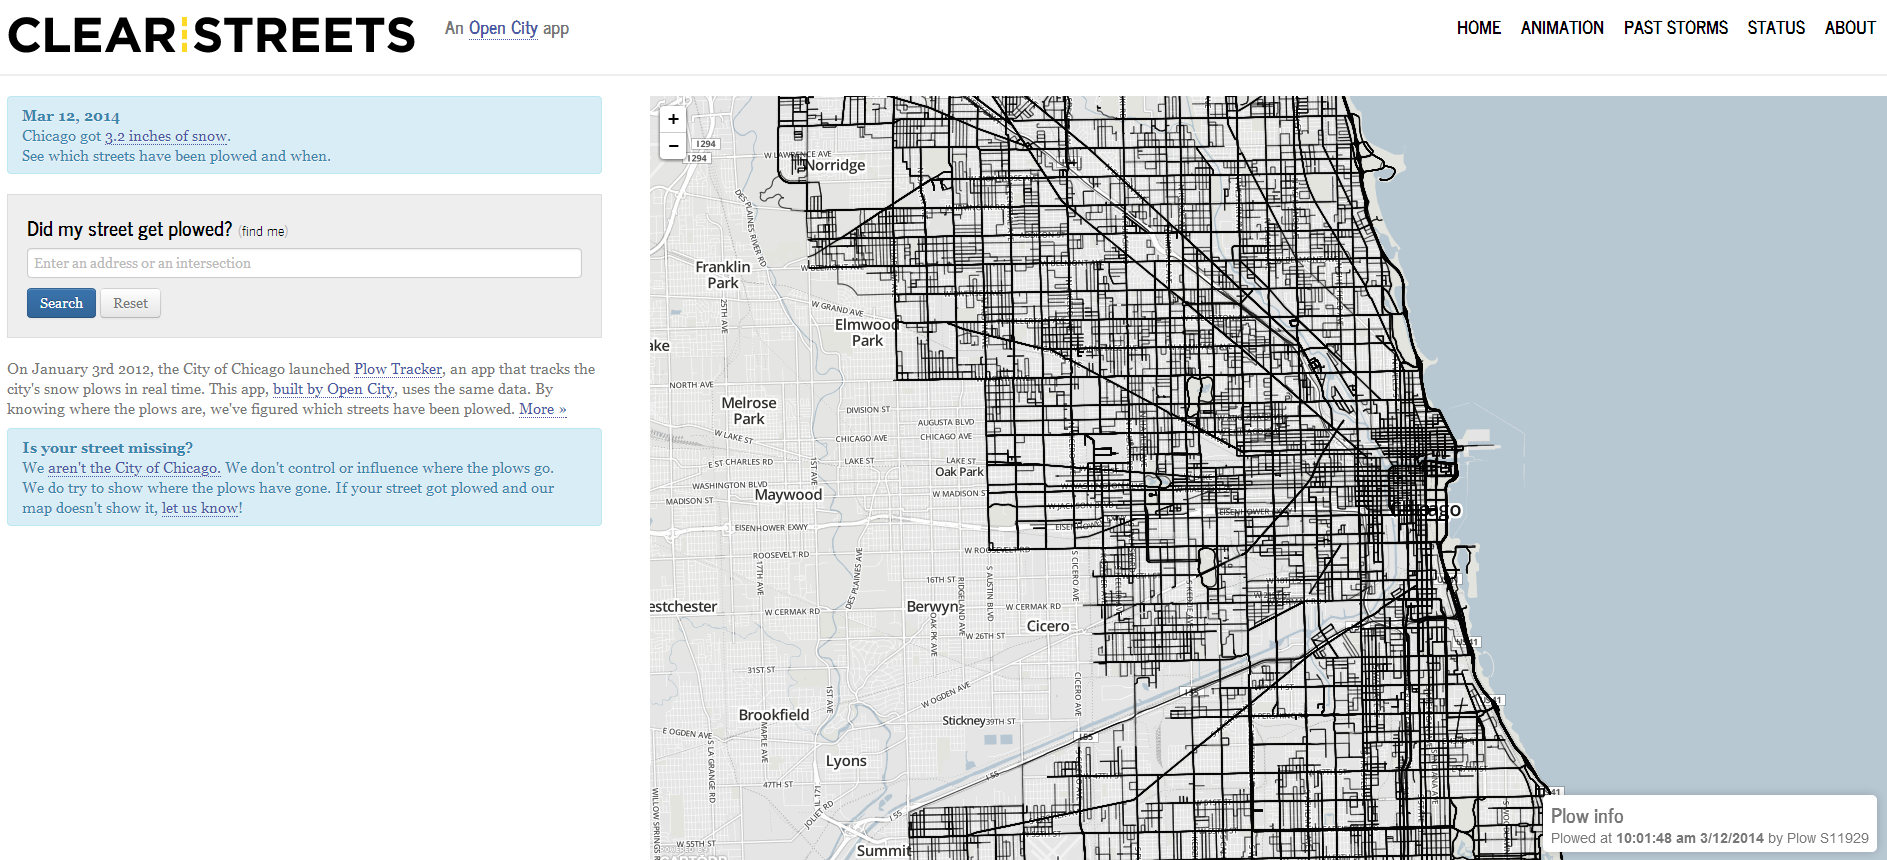
\includegraphics[scale=0.3]{clear_streets}
\caption{The clear streets website with a 'slippy' map}
\label{fig:clear_streets}
\end{figure}

Previously making maps of this type required specialist skills in spatial analysis and programming, and were almost exclusively made using the Google Maps \gls{api} which allows use of the Google Maps base layer to then add your own data on top. However there has been a huge surge in mapping products over the last five to ten years as the profitability and usage of geographical data has become clear and commonplace. As the field is rapidly evolving most books or review articles are out-of-date within weeks of publication, and therefore the following list of providers of global web-based slippy maps is taken from Wikipedia (\cite{wiki-maps-2014}):

\begin{itemize}
\item OpenStreetMap  (\url{http://www.openstreetmap.org/})
\item ArcGIS Online (Esri)  (\url{http://www.arcgis.com/home/webmap})
\item Google Maps \url{https://www.google.com/maps/})
\item Bing Maps (\url{http://www.bing.com/maps/})
\item MapQuest (\url{http://www.mapquest.com/})
\item WikiMapia (\url{http://wikimapia.org/})
\item HERE (\url{http://here.com/})
\item Mappy (\url{http://en.mappy.com/})
\item Yahoo! Maps (\url{https://maps.yahoo.com/})
\end{itemize}

Of this list the most popular and widely used are Google Maps and OpenStreetMap, however in following with the earlier stated aim of using FOSS tools, I decided to use OpenStreetMap background data for making online maps where needed in this research, due to it's community-made nature and lack of any restrictions on it's use or frequency of use.

To be able to use OpenStreetMap data as a background map with overlaps of data that are produced during this research, further tools are needed. The two introduced below are both FOSS4G implementations of the javascript programming language. 

\begin{itemize}
\item CartoDB.com (figure \ref{fig:cartodb_screen}): CartoDB is a cloud-based web-mapping, analysis and visualisation service. It allows storage of geographical data on their servers which can then be visualised on a map and published to a webpage. The advantages of CartoDB are the simplicity of producing professional looking maps with very little effort, however the amount of data that can be stored is limited without having to pay for additional storage. Despite this, for ad-hoc visualisations and/or ones that do not require a large amount of data to be displayed, this tool is very useful. CartoDB.com users can select OpenStreetMap data as the background for the maps that it serves to the users and can be easily customised.
\item Leaflet.js: Leaflet prides itself as a lightweight javascript library which displays, amongst a selection of others, OpenStreetMap data. By lightweight the community developers emphasise the very small amount of coding and expertise that is required to produce a map. Adding data and creating visualisations on top of the map is then of moderate difficulty. The main difference between CartoDB and Leaflet is that leaflet does not store the data, the webpage is coded so that the data is fed to it from another source such as an API, GeoJSON or CSV file. This has the advantage of there being no data-storage limits as the developer is responsible for the data themselves, however the knowledge and skills required to put the data onto the map are more advanced than that of using CartoDB.
\end{itemize}

\begin{figure}[H]
\centering
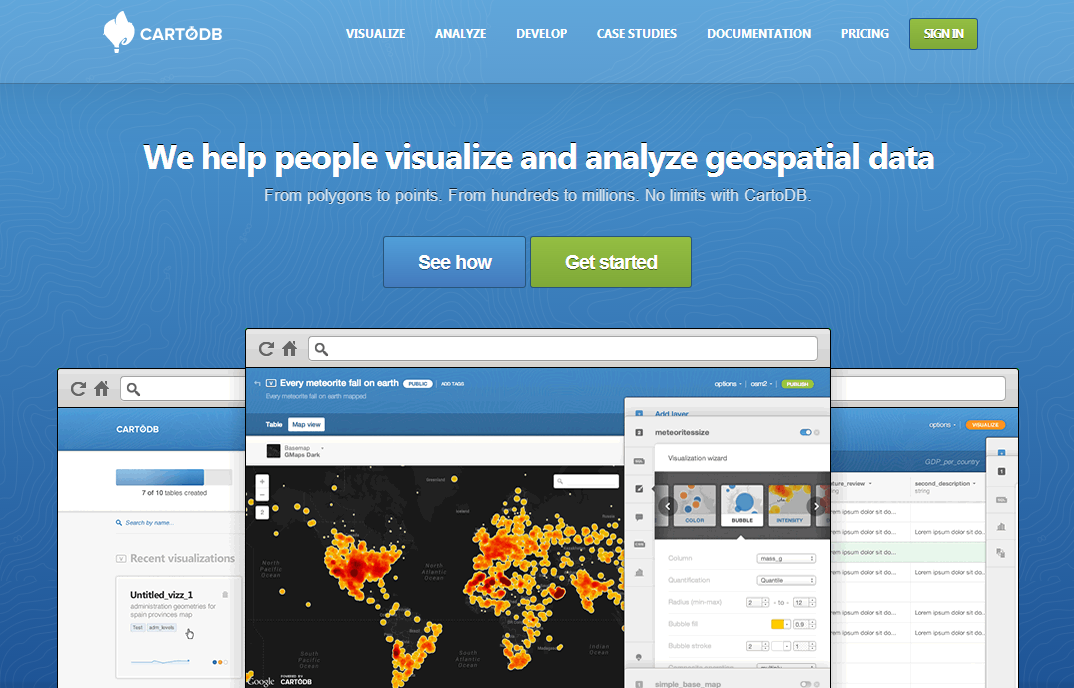
\includegraphics[scale=0.3]{cartodb_screen}
\caption{The CartoDB data visualisation platform}
\label{fig:cartodb_screen}
\end{figure}

When outputs of this research are required that are not suitable for a map, then graphs and charts using the plotting functionality of the \gls{foss} 'R' project (\cite{RFoundationforStatisticalComputing2014}), particularly the ggplot2 (\cite{ggplot2}) library will be used. One of the benefits of using R is that it can be easily connected to PostgreSQL, and statistical analysis and publication-quality plots can be produced with relative ease.

\end{comment}